\documentclass[conference]{IEEEtran}
% DRAFT v0.1 (23 Nov 2026). Every number comes from results/ via paper/make_paper_tables.py or is quoted from
% results/*.md; see paper/PAPER_PROMPT.md for the claim rules. Compile on Overleaf: upload the paper/ folder,
% main.tex as the main file, pdfLaTeX. References are in references.tex (generated by paper/make_references.py).
\usepackage[T1]{fontenc}
\usepackage[utf8]{inputenc}
\usepackage{cite}
\usepackage{amsmath,amssymb}
\usepackage{graphicx}
\usepackage{booktabs}
\usepackage{xcolor}
\usepackage{url}
\usepackage[hidelinks]{hyperref}
\graphicspath{{figs/}}
\newcommand{\todo}[1]{\textcolor{red}{[TODO: #1]}}

\begin{document}

\title{Recipe-Supervised Concepts for Robust and Explainable\\ Deepfake Detection: A Leak-Free Study}

\author{
\IEEEauthorblockN{Charan L, Deepak S N, Samrudh N Shindhe, Samarth Gowda G M, and Jyothi R}
\IEEEauthorblockA{Department of Computer Science and Engineering, PES University, Bengaluru, India\\
\{email\} \quad Corresponding author: Jyothi R, \{email\}}
}

\maketitle

\begin{abstract}
Face-forgery detectors trained on FaceForensics++ (FF++) lose accuracy on unseen datasets and compressed video,
and explain themselves with heatmaps of unknown faithfulness. We study these problems under a leak-free protocol:
identity-disjoint splits, leakage tests, selection on FF++ validation only, and three seeds with bootstrap
confidence intervals. Our detector, GRACE,
combines a LoRA-tuned CLIP ViT-L/14 with a block-DCT branch and a ten-concept bottleneck whose labels are read off
the recipe that synthesises each self-blended training fake, so concept supervision costs nothing. On DFD and
Celeb-DF (official test list), cross-dataset video AUC rises from 0.854 (Swin-B) to 0.914; most of this gain comes
from the CLIP backbone, and the GRACE additions do not significantly change clean AUC (+0.009, 95\% CI
[$-$0.007, +0.024]). They do keep accuracy under JPEG-30 compression (0.901 vs.\ 0.789), lower video-level
calibration error on Celeb-DF from 0.527 to 0.161, and give region maps that remove evidence as fast as the true
blend mask in a restoration test (0.281 vs.\ 0.270; random 0.663). Single-frame H.264 augmentation raises AUC at
CRF~40 from 0.644 to 0.688 at no clean cost. A distilled 4.7\,M-parameter student runs in 4.2\,ms per face on a CPU
but does not match the teacher. Domain-adversarial training hurt in every form we tried.
\end{abstract}

\begin{IEEEkeywords}
deepfake detection, concept bottleneck, self-blended images, CLIP, explainability, knowledge distillation
\end{IEEEkeywords}

% =====================================================================================================
\section{Introduction}

Face-manipulation detectors are usually trained on FaceForensics++ (FF++)~\cite{ffpp} and tested on datasets they
never saw, such as Google's DeepFakeDetection (DFD)~\cite{dfd} and Celeb-DF~\cite{celebdf}. Three gaps stand out
in this setting. First, \emph{generalisation}: in-domain AUC is close to 1.0 for almost any modern backbone, while
cross-dataset AUC falls well below it~\cite{deepfakebench,df40}. Second, \emph{robustness}: real videos are
re-compressed by platforms, and detectors that rely on fine high-frequency traces lose them under JPEG or H.264
compression. Third, \emph{explanation}: most systems justify a verdict with Grad-CAM~\cite{gradcam} or attention
rollout~\cite{rollout}, whose faithfulness is rarely measured and, when measured, often poor~\cite{tsigos}.

A fourth, less visible problem affects all three: evaluation leakage. Splitting FF++ by frame or by random video,
instead of by source identity, lets the same person appear in training and test data. Our own earlier checkpoint,
reported at 97.3\% validation accuracy, had trained on most of what later became our validation and test videos
(Section~\ref{sec:leak}).

We address these problems with GRACE, a detector whose decision passes through ten named forgery concepts. The
concept labels are free: self-blended images (SBI)~\cite{sbi} are pseudo-fakes made by blending a face with a
transformed copy of itself, and the parameters of that recipe (blend ratio, colour shift, blur, region, boundary
shape) are exactly the concepts we want the model to report. Our contributions are:
\begin{itemize}
\item A leak-free protocol (identity-disjoint splits, leakage tests, validation-only selection, 3 seeds, bootstrap
CIs over videos) and a case study of what leakage did to an earlier result.
\item A concept-bottleneck detector supervised by the SBI recipe, with a step-by-step ablation in which every
addition is tested against its parent model with paired confidence intervals.
\item Evidence that the concept maps are faithful when evidence is truly removed: a \emph{restoration} test that
restores real pixels, replacing the usual blur-based deletion test, which can add rather than remove forgery cues.
\item Robustness, calibration and distillation results, including a single-frame H.264 augmentation and a
65$\times$ smaller student, with negative results reported alongside.
\end{itemize}
We do not claim state-of-the-art accuracy: we train on a reduced FF++ subset (Section~\ref{sec:data}), and published
numbers use more data under different protocols.

% =====================================================================================================
\section{Related Work}

\textbf{Benchmarks and protocol.} FF++~\cite{ffpp}, Celeb-DF~\cite{celebdf}, DFD~\cite{dfd} and DFDC~\cite{dfdc}
are the standard datasets; DeepfakeBench~\cite{deepfakebench} and DF40~\cite{df40} unify training and evaluation
code and show how much results depend on protocol details.

\textbf{Synthetic training fakes.} Face X-ray~\cite{facexray} trains on blended faces and predicts the blending
boundary; SBI~\cite{sbi} blends a face with a transformed copy of itself, which removes identity cues and gives
strong cross-dataset results. We reuse the SBI idea but log every recipe parameter as a concept label.

\textbf{Foundation-model detectors.} UnivFD~\cite{univfd} showed that a linear probe on frozen CLIP~\cite{clip}
features generalises across generators. Later work adapts CLIP with adapters or constrained fine-tuning:
Forensics Adapter~\cite{fa}, orthogonal subspace decomposition (Effort)~\cite{effort}, and LayerNorm-only tuning
of CLIP~\cite{lnclip}. We use LoRA~\cite{lora} on the attention projections of a frozen CLIP ViT-L/14.

\textbf{Explanations.} Concept bottleneck models~\cite{cbm} predict human-named concepts and decide from them.
For deepfakes, Vanian et al.~\cite{whyfake} probe the semantic vocabulary of detectors, and
\cite{mansoor,dfp2e,laylens} build explanations for end users. Tsigos et al.~\cite{tsigos} evaluate saliency
methods quantitatively and find large differences. Our concepts differ in that their labels come from the
data-synthesis recipe, not from annotators or language models.

\textbf{Distillation and domain alignment.} Knowledge distillation~\cite{hinton} transfers a teacher's outputs
to a small student; domain-adversarial training~\cite{ganin} and MMD~\cite{mmd} align feature distributions across
domains and have been used for deepfake generalisation~\cite{irm}.

% =====================================================================================================
\section{Protocol}\label{sec:protocol}

\subsection{Data}\label{sec:data}
We use FF++ c23 real videos and the Deepfakes, Face2Face and FaceSwap manipulations available to us. The subset is
unbalanced: of 1,445 training videos, 719 are real and 611 Deepfakes, but only 90 are Face2Face and 25 FaceSwap.
Validation has 286 videos and test 280. DFD (1,274 test videos: 911 fake, 363 real) and Celeb-DF (official test
list, 516 of 518 videos usable: 340 Celeb-synthesis, 107 Celeb-real, 69 YouTube-real) are used only for testing.
Faces are detected with SFD and aligned with FAN~\cite{fan}; we use about 32 face crops of 224$\times$224 pixels per
video. A video's score is the mean fake probability of its frames, and we report video-level AUC.

\subsection{Splits, selection and statistics}
FF++ is split by source identity, so the people in validation and test never appear in training; automated tests
check that no video or FF++ source identity occurs in two splits and that no DFD or Celeb-DF video is used in
training. All choices (epoch, final model,
calibration temperature, decision threshold) use FF++ validation data only. The final model is chosen by the mean
of three validation scores: clean video AUC, video AUC on H.264 CRF-40 re-encoded validation videos, and AUC on
self-blended validation images. Each test set is evaluated after training finishes. Every model is trained with
seeds 42, 1 and 2. For each number we report the seed mean, and a 95\% confidence interval from 1,000 bootstrap
resamples of the test \emph{videos}, stratified by label; paired comparisons resample the same videos for both
models. \emph{Cross} denotes the mean AUC over DFD and Celeb-DF.

\subsection{Degradations}
Test frames are degraded by JPEG re-encoding (quality 90 to 30), downscaling (to 50\% or 25\% and back), and
H.264 encoding of each video's crops as an MP4 at CRF 28, 34 and 40 (libx264, 25\,fps).

\subsection{Leakage case study}\label{sec:leak}
An earlier version of our system was trained with a random video split over all available FF++ and DFD face
folders and reported 97.3\% validation accuracy. Evaluated on our leak-free splits, the same checkpoint scores
1.000 on FF++ validation and test and 0.999 on DFD, because it had trained on most of those videos. These numbers
are meaningless; only its Celeb-DF AUC (0.956), a dataset it never saw, is a fair figure, and it reflects the extra
training data (all of FF++ and DFD) rather than the method (Section~\ref{sec:disc}).

% =====================================================================================================
\section{Method}\label{sec:method}

\begin{figure}[t]
\centering
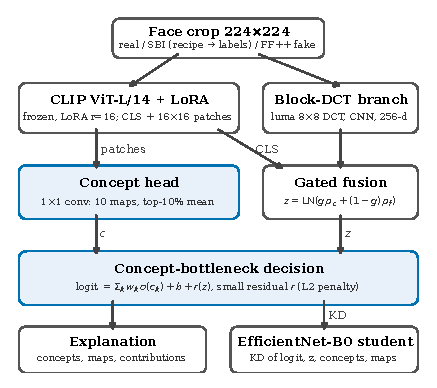
\includegraphics[width=\columnwidth]{fig_architecture.pdf}
\caption{GRACE. The concept head reads CLIP patch tokens; the decision is a weighted sum of concept scores plus a
small residual from the fused CLIP+DCT feature. The student copies the teacher's logit, feature, concepts and
maps.}
\label{fig:arch}
\end{figure}

\subsection{Self-blended images with recipe labels}
For a real face with 68 landmarks, the SBI engine picks a region (full face 0.4, mouth 0.25, eyes and brows 0.2,
nose and cheeks 0.15) and fills its convex hull. With probability 0.5 the mask is elastically warped; it is then
blurred with a random odd kernel of size 3 to 31. A copy of the face receives at least one transform: a colour
shift (p=0.5), blur or sharpening (0.5), down-and-up resampling (0.4) or a small affine misalignment (0.4). The copy
is blended into the original with ratio $a\in\{0.25,0.5,0.75,1\}$:
$x' = x\,(1-a m) + \tilde{x}\,a m$. The recipe gives ten concept targets (Table~\ref{tab:concepts}) and a
16$\times$16 boundary map $4m(1-m)$, normalised to a maximum of 1.

\begin{table}[t]
\centering\footnotesize
\caption{The ten concepts and how each label is set from the SBI recipe ($a$: blend ratio).}
\label{tab:concepts}
\begin{tabular}{lll}
\toprule
& Concept & Label \\
\midrule
c1 & blend strength & $a$ \\
c2 & colour mismatch & $a\times$ colour-shift strength \\
c3 & blur & $a$ if the copy was blurred, else 0 \\
c4 & sharpen & $a$ if sharpened \\
c5 & resampling & $a$ if resampled \\
c6 & mouth region & 1 if region = mouth \\
c7 & eye region & 1 if region = eyes and brows \\
c8 & full face & 1 if region = full face \\
c9 & geometric misalignment & $a$ if affine shift applied \\
c10 & irregular boundary & 1 if the mask was warped \\
\bottomrule
\end{tabular}
\end{table}

\subsection{Architecture}
Fig.~\ref{fig:arch} shows the model. \textbf{Backbone.} CLIP ViT-L/14 at 224 pixels, frozen, with LoRA (rank 16, $\alpha$=32, dropout 0.1) on the
attention \texttt{qkv} projections. It outputs a CLS feature and a 16$\times$16 grid of patch tokens.

\textbf{Frequency branch.} The luminance image is split into 8$\times$8 blocks and transformed with an orthonormal
DCT-II, the transform used by JPEG and H.264. Log-magnitudes of the 64 coefficients pass through a small CNN to a
256-d feature.

\textbf{Gated fusion.} With $p_c$ and $p_f$ the projections of the CLS and frequency features to 512-d,
$g=\sigma(W[p_c;p_f])$ and $z=\mathrm{LN}(g\odot p_c+(1-g)\odot p_f)$.

\textbf{Concept bottleneck.} A 1$\times$1 convolution maps the patch grid to ten concept maps; the score $c_k$ is
the mean of the top 10\% of cells of map $k$. The decision is
\begin{equation}
\ell = \sum_{k=1}^{10} w_k\,\sigma(c_k) + b + r(z),
\end{equation}
where $r$ is a two-layer MLP whose last layer starts at zero. The residual lets the frequency feature, which the
concept head does not see, reach the decision; an L2 penalty keeps it small.

\subsection{Training objective}
Each batch mixes real faces, SBI fakes and FF++ fakes (sampling weights 3:2:1:1:1 for real, SBI, Deepfakes,
Face2Face, FaceSwap). With $\mathcal{B}$ the binary cross-entropy,
\begin{equation}
\mathcal{L} = \mathcal{B}(\ell,y) + \lambda_c\,\mathcal{B}_{\mathrm{SBI}}(c,\hat c)
+ \lambda_m\,\mathcal{B}_{\mathrm{SBI}}(M,\hat M) + \lambda_w\|w\|_1 + \lambda_r\,\overline{r(z)^2},
\end{equation}
where concept and map terms apply only to SBI images (FF++ fakes have no recipe), $M$ is the concept-map output
compared with the boundary map, $\lambda_c=\lambda_m=0.5$, $\lambda_w=10^{-4}$ and $\lambda_r=10^{-2}$.
We train with AdamW~\cite{adamw} (weight decay 0.05; learning rates $2\times10^{-4}$ for LoRA, $10^{-3}$ for heads,
$2\times10^{-3}$ for the DCT branch), 12 epochs of 1,500 steps, batch 32, bf16, one warm-up epoch and an EMA of the
weights (0.999). Augmentation: flip, colour jitter, blur, and JPEG (p=0.3, quality 60--100). Training one model
takes about two hours on one NVIDIA RTX 4500 Ada GPU.

\textbf{H.264 augmentation (F1h).} With probability 0.3, a training crop is encoded as a single H.264 frame
(libx264, CRF drawn from 24--38) and decoded back. This is intra-only and approximates, but is not the same as, the
video-level test encoding; CRF 40 is never used in training.

\subsection{Distillation}
The student is an EfficientNet-B0~\cite{efficientnet} with the same concept head on its 7$\times$7 feature grid. It
trains on degraded frames (clean 0.2, JPEG q20--60 0.35, downscale 0.25--0.5 0.25, both 0.2) while reading the
teacher's outputs on the clean frame from a cache:
\begin{equation}
\mathcal{L}_S = 0.5\,\mathcal{B} + 0.5\,T^2\mathrm{KL}_T + \|z_S-z_T\|^2 + 0.5\,\mathcal{B}(c_S,\sigma(c_T))
+ 0.5\,\|\sigma(M_S)-\sigma(M_T)\|^2,
\end{equation}
with temperature $T=4$. S0 is the same student without a teacher; S3h adds single-frame H.264 to a quarter of the
degraded inputs.

\subsection{Baselines}
\textbf{B1}: Swin-B~\cite{swin} fine-tuned on FF++ fakes. \textbf{R1}: UnivFD-style~\cite{univfd} linear probe on
frozen CLIP ViT-L/14. \textbf{R2}: our reproduction of SBI~\cite{sbi}, EfficientNet-B4 trained on real faces and
their self-blends only, using our SBI engine and data. \textbf{C1}: CLIP+LoRA with a linear head. All share our
splits, face crops, selection rule and evaluation code.

% =====================================================================================================
\section{Results}\label{sec:results}

\begin{table*}[t]
\centering
\footnotesize
\caption{Video AUC under the leak-free protocol (mean$\pm$sample std over 3 seeds). Cross is the mean of the DFD and Celeb-DF AUCs; its 95\% CI comes from 1,000 stratified bootstrap resamples of the test videos applied to the seed-mean AUC. All models share the FF++ training videos, face crops, sampler and selection code; R2 trains on real faces and their self-blends only.}
\label{tab:main}
\begin{tabular}{llccccc}
\toprule
ID & Model & FF++ test & DFD & Celeb-DF & Cross & Cross 95\% CI \\
\midrule
B1 & Swin-B, FF++ fakes & 0.997$\pm$0.003 & 0.903$\pm$0.020 & 0.805$\pm$0.016 & 0.854$\pm$0.012 & [0.837, 0.872] \\
R1 & frozen CLIP, linear probe & 0.944$\pm$0.000 & 0.857$\pm$0.001 & 0.743$\pm$0.002 & 0.800$\pm$0.001 & [0.775, 0.825] \\
R2 & SBI reprod., EffNet-B4 & 0.906$\pm$0.008 & 0.810$\pm$0.009 & 0.616$\pm$0.015 & 0.713$\pm$0.009 & [0.684, 0.742] \\
\midrule
C1 & CLIP ViT-L/14 + LoRA & 1.000$\pm$0.000 & 0.931$\pm$0.010 & 0.880$\pm$0.011 & 0.906$\pm$0.009 & [0.892, 0.920] \\
F1 & final teacher & 0.997$\pm$0.004 & 0.951$\pm$0.004 & 0.878$\pm$0.017 & 0.914$\pm$0.010 & [0.898, 0.930] \\
F1h & F1 + H.264 augmentation & 0.993$\pm$0.007 & 0.939$\pm$0.006 & 0.886$\pm$0.005 & 0.912$\pm$0.004 & [0.896, 0.928] \\
\bottomrule
\end{tabular}
\end{table*}


\subsection{Main comparison}
Table~\ref{tab:main} gives the main results. All models are near-perfect on FF++ test, so the cross-dataset
columns carry the comparison. F1 improves on the Swin-B baseline by +0.060 cross AUC (95\% CI [+0.042, +0.079]),
on the frozen-CLIP probe R1 by +0.114, and on our SBI reproduction R2 by +0.201. R2 is far below the Celeb-DF
result reported by its authors~\cite{sbi}, who trained on all of FF++ with their own pipeline; we report it only as
a reference under our data and budget. Against C1, which shares the backbone, the difference is +0.009
(CI [$-$0.007, +0.024], $p$=0.31): on clean video, the backbone change accounts for the gain.

\begin{table*}[t]
\centering
\footnotesize
\caption{Paired change in seed-mean video AUC, later model minus earlier (3 seeds each, the same resampled videos for both models). $^{*}$: the 95\% paired bootstrap CI excludes zero. CI and two-sided bootstrap $p$ refer to the cross column. Concept share: variance of the concept part of the logit divided by the variance of the logit on FF++ test frames, for the later model (-- for linear heads).}
\label{tab:ablation}
\begin{tabular}{llcccccc}
\toprule
Pair & Change & DFD & Celeb-DF & Cross & Cross 95\% CI & $p$ & Concept share \\
\midrule
C2 vs.\ C1 & + SBI pseudo-fakes in the batch & +0.028$^{*}$ & $-$0.023 & +0.003 & [$-$0.014, +0.019] & 0.752 & -- \\
G1 vs.\ C2 & + concept bottleneck (residual 1e-3) & $-$0.004$^{*}$ & +0.022$^{*}$ & +0.009$^{*}$ & [+0.004, +0.014] & 0.000 & 0.36$\pm$0.15 \\
G2 vs.\ G1 & + block-DCT branch, gated fusion & +0.010$^{*}$ & +0.002 & +0.006$^{*}$ & [+0.002, +0.010] & 0.000 & 0.36$\pm$0.13 \\
F1 vs.\ G2 & residual 1e-3 $\to$ 1e-2, harder selection & $-$0.015$^{*}$ & $-$0.003 & $-$0.009$^{*}$ & [$-$0.017, $-$0.001] & 0.022 & 0.84$\pm$0.00 \\
G3 vs.\ A3 & concept head vs.\ linear head (both + DANN) & +0.013$^{*}$ & +0.019$^{*}$ & +0.016$^{*}$ & [+0.006, +0.025] & 0.000 & 1.00$\pm$0.00 \\
\midrule
C1 vs.\ B1 & Swin-B $\to$ CLIP ViT-L/14 + LoRA & +0.028$^{*}$ & +0.075$^{*}$ & +0.052$^{*}$ & [+0.037, +0.067] & 0.000 & -- \\
F1 vs.\ C1 & all additions together & +0.019$^{*}$ & $-$0.002 & +0.009 & [$-$0.007, +0.024] & 0.308 & 0.84$\pm$0.00 \\
F1h vs.\ F1 & + single-frame H.264 augmentation & $-$0.011$^{*}$ & +0.008 & $-$0.002 & [$-$0.008, +0.004] & 0.588 & 0.81$\pm$0.00 \\
\bottomrule
\end{tabular}
\end{table*}


\subsection{Ablation}
Table~\ref{tab:ablation} tests each step against its parent. Adding SBI fakes to C1 raises DFD but lowers Celeb-DF,
with no net cross-dataset change. The concept bottleneck (G1) adds +0.009 and the DCT branch (G2) +0.006, both
significant. F1 trades 0.009 of cross AUC against G2 for its harder selection rule and residual penalty; we keep
it because it was chosen on validation data before any test number was seen, and it is the most robust model under
compression (Table~\ref{tab:robust}). The cleanest test of the bottleneck is A3 against G3, which differ only in the
head: the concept head is better by +0.016 (CI [+0.006, +0.025]) and is significant on both test sets.

\begin{table}[t]
\centering
\footnotesize
\setlength{\tabcolsep}{3pt}
\caption{Cross-dataset video AUC with degraded test frames (mean$\pm$sample std, 3 seeds). Down 0.25: downscale to 25\% and back. F1h trains with CRF 24--38, never 40.}
\label{tab:robust}
\begin{tabular}{lcccc}
\toprule
Model & Clean & JPEG 30 & Down 0.25 & H.264 40 \\
\midrule
B1 & 0.854$\pm$0.012 & 0.776$\pm$0.033 & 0.757$\pm$0.030 & 0.561$\pm$0.012 \\
R1 & 0.800$\pm$0.001 & 0.757$\pm$0.001 & 0.741$\pm$0.000 & 0.681$\pm$0.001 \\
R2 & 0.713$\pm$0.009 & 0.710$\pm$0.011 & 0.719$\pm$0.010 & 0.555$\pm$0.014 \\
\midrule
C1 & 0.906$\pm$0.009 & 0.789$\pm$0.026 & 0.823$\pm$0.012 & 0.624$\pm$0.014 \\
C2 & 0.908$\pm$0.003 & 0.898$\pm$0.017 & 0.886$\pm$0.007 & 0.661$\pm$0.018 \\
G1 & 0.917$\pm$0.004 & 0.901$\pm$0.005 & 0.895$\pm$0.013 & 0.652$\pm$0.011 \\
G2 & 0.923$\pm$0.009 & 0.909$\pm$0.008 & 0.895$\pm$0.014 & 0.653$\pm$0.026 \\
F1 & 0.914$\pm$0.010 & 0.901$\pm$0.008 & 0.878$\pm$0.010 & 0.644$\pm$0.020 \\
F1h & 0.912$\pm$0.004 & 0.894$\pm$0.003 & 0.875$\pm$0.009 & 0.688$\pm$0.006 \\
\bottomrule
\end{tabular}
\end{table}


\begin{figure}[t]
\centering
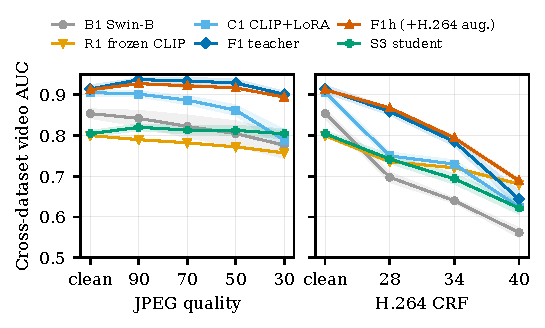
\includegraphics[width=\columnwidth]{fig_robustness.pdf}
\caption{Cross-dataset video AUC as test compression grows (bands: $\pm$1 std over 3 seeds).}
\label{fig:robust}
\end{figure}

\subsection{Robustness}
Under JPEG-30, C1 falls from 0.906 to 0.789 while F1 stays at 0.901 (Table~\ref{tab:robust},
Fig.~\ref{fig:robust}). Strong H.264 compression is the hardest condition for every model: at CRF 40 F1 reaches
only 0.644. Single-frame H.264 augmentation (F1h) raises this to 0.688 (paired +0.045, CI [+0.025, +0.063]) with no
significant clean change ($-$0.002, CI [$-$0.008, +0.004]), and also lowers the seed spread. Interestingly, the
frozen probe R1 is the second most robust model at CRF 40 (0.681): frozen features lose less under compression,
although they rank clean videos worse. Students do not gain from H.264 inputs at CRF 40 (S3h 0.610 vs.\ S3 0.622,
not significant), though S3h is better on clean DFD.

\subsection{Explanations}
\begin{table}[t]
\centering
\footnotesize
\setlength{\tabcolsep}{3pt}
\caption{Explanation quality on held-out self-blended test images with known blend masks. Pointing game and mask IoU: higher is better ($n$=2,000; region concept $n$=1,713). Blur-deletion and restoration: area under the fake-probability curve as patches are blurred or restored to the real source pixels, lower is better ($n$=500 images the teacher flags; region concept $n$=438). B1 and C1 do not flag these images (mean start probability 0.15 and 0.24), so their restoration curves are not comparable and are omitted.}
\label{tab:explain}
\begin{tabular}{lcccc}
\toprule
Map & Pointing$\uparrow$ & IoU$\uparrow$ & Blur-del.$\downarrow$ & Restore$\downarrow$ \\
\midrule
F1 region concept & 0.938 & 0.384 & -- & 0.281 \\
F1 blend-strength map & 0.517 & 0.225 & 0.984 & 0.494 \\
S3 blend-strength map & 0.725 & 0.259 & 0.923 & 0.544 \\
B1 Grad-CAM & 0.155 & 0.052 & 0.702 & -- \\
C1 attention rollout & 0.013 & 0.016 & 0.775 & -- \\
Random map & 0.246 & 0.067 & 0.908 & 0.663 \\
Oracle (true mask) & -- & -- & -- & 0.270 \\
\bottomrule
\end{tabular}
\end{table}


We measure explanations on held-out self-blended test images, where the true blend mask is known
(Table~\ref{tab:explain}). The region concept of F1 (mouth, eyes or full face, chosen by the true region) hits the
mask in 93.8\% of images, against 15.5\% for Grad-CAM on B1 and 1.3\% for attention rollout on C1. The student's
blend-strength map points better than the teacher's (0.725 vs.\ 0.517), because its coarser 7$\times$7 grid spreads
over the face.

\textbf{Deletion versus restoration.} In the usual deletion test, patches are replaced by a blurred copy in order
of importance. Here F1's map is \emph{worse} than random (0.984 vs.\ 0.908). Blur, however, is one of the forgery
cues the model was trained to detect, so blurring a patch can add evidence. Because each SBI test image has a known
real source frame, we can instead \emph{restore} patches to their real pixels, which removes evidence by
construction. Under restoration, F1's region map lowers the fake probability almost exactly as fast as the true
mask (0.281 vs.\ 0.270) and far faster than random order (0.663); the blend-strength maps of F1 and S3 also beat
random. We therefore read the deletion failure as a property of the test rather than of the maps, while noting that
restoration is only possible on synthetic fakes.

\textbf{Interventions.} Switching off the top concept lowers F1's fake probability by 0.054 on average, against
0.011 for a random concept (S3: 0.022 vs.\ 0.005).

\textbf{Concepts on real forgeries.} The concepts were learned only from SBI images, yet they respond sensibly to
real manipulations. The mean ``full face'' score is 0.43 on Celeb-DF fakes and 0.66 on DFD fakes, against 0.08--0.13
on real videos of the same datasets; on FF++, Face2Face and FaceSwap raise the eye-region concept (0.45 and 0.41)
far more than Deepfakes (0.14). Nine of the ten concepts are learned (concept AUC 0.76--1.00 on SBI test images);
the irregular-boundary concept c10 is not (0.515).

\begin{table}[t]
\centering
\footnotesize
\setlength{\tabcolsep}{3pt}
\caption{Expected calibration error of the video score (15 equal-width bins, seed 42; lower is better), raw / after the temperature $T$ fitted on FF++ validation frames.}
\label{tab:ece}
\begin{tabular}{lcccc}
\toprule
Model & $T$ & FF++ & DFD & Celeb-DF \\
\midrule
B1 & 4.75 & 0.057 / 0.089 & 0.237 / 0.233 & 0.578 / 0.489 \\
R1 & 1.00 & 0.093 / 0.093 & 0.182 / 0.182 & 0.394 / 0.394 \\
R2 & 1.00 & 0.151 / 0.151 & 0.067 / 0.067 & 0.088 / 0.088 \\
C1 & 1.00 & 0.037 / 0.037 & 0.261 / 0.261 & 0.527 / 0.527 \\
C2 & 1.00 & 0.082 / 0.082 & 0.075 / 0.075 & 0.069 / 0.069 \\
G1 & 1.00 & 0.108 / 0.108 & 0.158 / 0.158 & 0.230 / 0.230 \\
G2 & 1.00 & 0.107 / 0.107 & 0.157 / 0.157 & 0.216 / 0.216 \\
F1 & 1.04 & 0.068 / 0.071 & 0.075 / 0.074 & 0.161 / 0.159 \\
F1h & 1.00 & 0.075 / 0.075 & 0.048 / 0.048 & 0.059 / 0.059 \\
S3 & 1.66 & 0.074 / 0.121 & 0.074 / 0.071 & 0.105 / 0.075 \\
\bottomrule
\end{tabular}
\end{table}


\subsection{Calibration}
Table~\ref{tab:ece} reports the expected calibration error~\cite{guo} of the raw probabilities. On Celeb-DF, B1 and
C1 are badly over- or under-confident (0.578, 0.527), while F1 reaches 0.161 and F1h 0.059. Temperature scaling fitted on
FF++ validation helps little (B1 on Celeb-DF: 0.578$	o$0.489), because FF++ validation is almost perfectly
separated. ECE measures whether probabilities can be read
as frequencies, not ranking quality: R2 is well calibrated but ranks poorly.

\subsection{Distillation and efficiency}
The student has 4.71\,M parameters and 0.39\,GFLOPs, against 306.94\,M and 81.46\,GFLOPs for F1 (65$\times$
fewer), and runs in 4.2\,ms per face as ONNX on a CPU with 4 threads (batch 1). Its cross AUC is 0.804, well below the
teacher's 0.914. Full distillation does not beat the teacher-free S0 on clean data ($-$0.005, CI [$-$0.014,
+0.005]); its benefit is behavioural: concept agreement with the teacher rises from Spearman $\rho$=0.683 (S0) to
0.767 (S3), and the seed spread halves.

\subsection{What did not work}
Domain-adversarial training lowered cross AUC every time: on Swin-B with real faces as a domain (0.854$\to$0.828),
on the fused feature of the teacher (G3; 0.915$\to$0.912 vs.\ its FFT parent), and on patch features (F2, 0.733).
Unsupervised adaptation to unlabelled Celeb-DF videos lowered Celeb-DF AUC from 0.878 to 0.832. An FFT frequency
branch was worse than the DCT branch (0.915, one seed, vs.\ 0.923).

\subsection{Failure analysis}
On Celeb-DF, F1 separates fakes from Celeb-real videos well (AUC 0.920) but from YouTube-real videos less well
(0.832). Of its 15 most confident errors, 13 are fakes with very low image sharpness scored as real and two are
YouTube-real videos scored as fake. AUC is highest on the sharpest third of videos (0.943) and lower on the least sharp (0.888).

% =====================================================================================================
\section{Discussion and Limitations}\label{sec:disc}

\textbf{Data diversity beats architecture.} The same G3 model trained on FF++ plus DFD reaches 0.944 on Celeb-DF
(3 seeds), against 0.860 when trained on FF++ alone and 0.878 for F1, a larger gain than any architectural change we
tested. The leaked earlier checkpoint, trained on more data, likewise scored 0.956 on Celeb-DF. The most useful next
step is the full FF++ release, which we are retraining on.

\textbf{What the additions buy.} On clean video, GRACE is statistically tied with CLIP+LoRA. Its value is that the
same accuracy comes with named concepts, maps that pass a restoration test, better calibration and much better
robustness to JPEG compression.

\textbf{Limitations.} We train on a reduced, unbalanced FF++ c23 subset with three manipulation types; we test on
two unseen datasets, both face-swap-heavy, and not on diffusion-generated or audio-driven forgeries. Restoration and
pointing-game results use synthetic fakes, where masks are known. Model selection uses an H.264 version of FF++
validation, so F1 is not blind to that degradation type, although the test videos are. The datasets are under
research licences and are not redistributed.

% =====================================================================================================
\section{Conclusion}
Under a leak-free protocol with three seeds and paired bootstrap intervals, a recipe-supervised concept bottleneck
on CLIP gives a detector that matches its CLIP+LoRA parent on clean cross-dataset AUC, is far more robust to JPEG
compression and better calibrated, and explains its decisions with concept maps that remove forgery evidence as fast
as the true mask. H.264 augmentation narrows, but does not close, the gap under strong video compression. Code,
configurations and per-video predictions are available at \url{https://github.com/pes1ug23cs178/CAPSTONE_PW_26_RJ_02}.

\section*{Acknowledgment}
We thank the Department of Computer Science and Engineering, PES University, for compute resources.
\todo{AI-use disclosure as required by the venue, e.g.\ ``An AI assistant was used to help draft and edit the text
and code; the authors checked all content and results.''}

\begin{thebibliography}{99}
\footnotesize
\bibitem{ffpp} A. Rössler, D. Cozzolino, L. Verdoliva, C. Riess, J. Thies, and M. Nießner, ``FaceForensics++: Learning to detect manipulated facial images,'' in \emph{Proc. IEEE/CVF Int. Conf. Computer Vision (ICCV)}, 2019, pp. 1--11.
\bibitem{dfd} N. Dufour and A. Gully, ``Contributing data to deepfake detection research,'' Google AI Blog, Sep. 24, 2019. [Online]. Available: \url{https://research.google/blog/contributing-data-to-deepfake-detection-research/}
\bibitem{celebdf} Y. Li, X. Yang, P. Sun, H. Qi, and S. Lyu, ``Celeb-DF: A large-scale challenging dataset for DeepFake forensics,'' in \emph{Proc. IEEE/CVF Conf. Computer Vision and Pattern Recognition (CVPR)}, 2020, pp. 3207--3216.
\bibitem{deepfakebench} Z. Yan, Y. Zhang, X. Yuan, S. Lyu, and B. Wu, ``DeepfakeBench: A comprehensive benchmark of deepfake detection,'' in \emph{Proc. Advances in Neural Information Processing Systems (NeurIPS), Datasets and Benchmarks Track}, 2023.
\bibitem{df40} Z. Yan, T. Yao, S. Chen, Y. Zhao, X. Fu, J. Zhu, D. Luo, C. Wang, S. Ding, Y. Wu, and L. Yuan, ``DF40: Toward next-generation deepfake detection,'' in \emph{Proc. Advances in Neural Information Processing Systems (NeurIPS), Datasets and Benchmarks Track}, 2024.
\bibitem{gradcam} R. R. Selvaraju, M. Cogswell, A. Das, R. Vedantam, D. Parikh, and D. Batra, ``Grad-CAM: Visual explanations from deep networks via gradient-based localization,'' in \emph{Proc. IEEE Int. Conf. Computer Vision (ICCV)}, 2017, pp. 618--626.
\bibitem{rollout} S. Abnar and W. Zuidema, ``Quantifying attention flow in transformers,'' in \emph{Proc. Annual Meeting of the Association for Computational Linguistics (ACL)}, 2020, pp. 4190--4197.
\bibitem{tsigos} K. Tsigos, E. Apostolidis, S. Baxevanakis, S. Papadopoulos, and V. Mezaris, ``Towards quantitative evaluation of explainable AI methods for deepfake detection,'' in \emph{Proc. ACM Int. Workshop on Multimedia AI against Disinformation (MAD '24)}, 2024, doi: 10.1145/3643491.3660292.
\bibitem{sbi} K. Shiohara and T. Yamasaki, ``Detecting deepfakes with self-blended images,'' in \emph{Proc. IEEE/CVF Conf. Computer Vision and Pattern Recognition (CVPR)}, 2022, pp. 18720--18729.
\bibitem{dfdc} B. Dolhansky, J. Bitton, B. Pflaum, J. Lu, R. Howes, M. Wang, and C. Canton Ferrer, ``The DeepFake Detection Challenge (DFDC) dataset,'' arXiv:2006.07397, 2020.
\bibitem{facexray} L. Li, J. Bao, T. Zhang, H. Yang, D. Chen, F. Wen, and B. Guo, ``Face X-ray for more general face forgery detection,'' in \emph{Proc. IEEE/CVF Conf. Computer Vision and Pattern Recognition (CVPR)}, 2020, pp. 5001--5010.
\bibitem{univfd} U. Ojha, Y. Li, and Y. J. Lee, ``Towards universal fake image detectors that generalize across generative models,'' in \emph{Proc. IEEE/CVF Conf. Computer Vision and Pattern Recognition (CVPR)}, 2023, pp. 24480--24489.
\bibitem{clip} A. Radford et al., ``Learning transferable visual models from natural language supervision,'' in \emph{Proc. Int. Conf. Machine Learning (ICML)}, 2021, pp. 8748--8763.
\bibitem{fa} X. Cui, Y. Li, A. Luo, J. Zhou, and J. Dong, ``Forensics Adapter: Adapting CLIP for generalizable face forgery detection,'' in \emph{Proc. IEEE/CVF Conf. Computer Vision and Pattern Recognition (CVPR)}, 2025, pp. 19207--19217.
\bibitem{effort} Z. Yan, J. Wang, P. Jin, K.-Y. Zhang, C. Liu, S. Chen, T. Yao, S. Ding, B. Wu, and L. Yuan, ``Orthogonal subspace decomposition for generalizable AI-generated image detection,'' in \emph{Proc. 42nd Int. Conf. Machine Learning (ICML)}, PMLR, vol. 267, 2025, pp. 70268--70288.
\bibitem{lnclip} A. Yermakov, J. Cech, J. Matas, and M. Fritz, ``Deepfake detection that generalizes across benchmarks,'' arXiv:2508.06248, 2025.
\bibitem{lora} E. J. Hu, Y. Shen, P. Wallis, Z. Allen-Zhu, Y. Li, S. Wang, L. Wang, and W. Chen, ``LoRA: Low-rank adaptation of large language models,'' in \emph{Proc. Int. Conf. Learning Representations (ICLR)}, 2022.
\bibitem{cbm} P. W. Koh, T. Nguyen, Y. S. Tang, S. Mussmann, E. Pierson, B. Kim, and P. Liang, ``Concept bottleneck models,'' in \emph{Proc. Int. Conf. Machine Learning (ICML)}, 2020, pp. 5338--5348.
\bibitem{whyfake} V. Vanian, A. Doumanoglou, and D. Zarpalas, ``Why fake? Unveiling the semantic vocabulary of deepfake detectors,'' in \emph{Proc. IEEE/CVF Conf. Computer Vision and Pattern Recognition Workshops (CVPRW)}, 2026, arXiv:2607.07216.
\bibitem{mansoor} N. Mansoor and A. I. Iliev, ``Explainable AI for DeepFake detection,'' \emph{Applied Sciences}, vol. 15, no. 2, Art. no. 725, Jan. 2025, doi: 10.3390/app15020725.
\bibitem{dfp2e} S. Tariq, S. S. Woo, P. Singh, I. Irmalasari, S. Gupta, and D. Gupta, ``From prediction to explanation: Multimodal, explainable, and interactive deepfake detection framework for non-expert users,'' in \emph{Proc. 33rd ACM Int. Conf. Multimedia (MM '25)}, 2025, doi: 10.1145/3746027.3755786.
\bibitem{laylens} A. Narang, P. Gupta, L. Su, and A. Dhall, ``LayLens: Improving deepfake understanding through simplified explanations,'' arXiv:2507.10066, 2025.
\bibitem{hinton} G. Hinton, O. Vinyals, and J. Dean, ``Distilling the knowledge in a neural network,'' arXiv:1503.02531, 2015.
\bibitem{ganin} Y. Ganin, E. Ustinova, H. Ajakan, P. Germain, H. Larochelle, F. Laviolette, M. Marchand, and V. Lempitsky, ``Domain-adversarial training of neural networks,'' \emph{J. Machine Learning Research}, vol. 17, no. 59, pp. 1--35, 2016.
\bibitem{mmd} A. Gretton, K. M. Borgwardt, M. J. Rasch, B. Schölkopf, and A. Smola, ``A kernel two-sample test,'' \emph{J. Machine Learning Research}, vol. 13, pp. 723--773, 2012.
\bibitem{irm} Z. Yin, J. Wang, Y. Xiao, H. Zhao, T. Li, W. Zhou, A. Liu, and X. Liu, ``Improving deepfake detection generalization by invariant risk minimization,'' \emph{IEEE Trans. Multimedia}, vol. 26, pp. 6785--6798, 2024, doi: 10.1109/TMM.2024.3355651.
\bibitem{fan} A. Bulat and G. Tzimiropoulos, ``How far are we from solving the 2D \& 3D face alignment problem? (and a dataset of 230,000 3D facial landmarks),'' in \emph{Proc. IEEE Int. Conf. Computer Vision (ICCV)}, 2017, pp. 1021--1030.
\bibitem{adamw} I. Loshchilov and F. Hutter, ``Decoupled weight decay regularization,'' in \emph{Proc. Int. Conf. Learning Representations (ICLR)}, 2019.
\bibitem{efficientnet} M. Tan and Q. V. Le, ``EfficientNet: Rethinking model scaling for convolutional neural networks,'' in \emph{Proc. Int. Conf. Machine Learning (ICML)}, 2019, pp. 6105--6114.
\bibitem{swin} Z. Liu, Y. Lin, Y. Cao, H. Hu, Y. Wei, Z. Zhang, S. Lin, and B. Guo, ``Swin Transformer: Hierarchical vision transformer using shifted windows,'' in \emph{Proc. IEEE/CVF Int. Conf. Computer Vision (ICCV)}, 2021, pp. 10012--10022.
\bibitem{guo} C. Guo, G. Pleiss, Y. Sun, and K. Q. Weinberger, ``On calibration of modern neural networks,'' in \emph{Proc. Int. Conf. Machine Learning (ICML)}, 2017, pp. 1321--1330.
\end{thebibliography}


\end{document}
